%\documentclass[]{article}
\documentclass[12pt]{article}

% my modifications:
\usepackage{fontspec}
\usepackage{booktabs}
\usepackage{mathptmx}
\defaultfontfeatures{Ligatures=TeX}
\setsansfont{Calibri}
\setmonofont{Inconsolata}
\setmainfont{Linux Libertine}
%\setmainfont{Times New Roman}
%\setmainfont{Calibri}
%\setmainfont{Helvetica}
\DeclareTextCommandDefault{\nobreakspace}{\leavevmode\nobreak\ }
\widowpenalty=1000
\clubpenalty=1000
\usepackage{setspace}
\onehalfspacing
%\doublespacing

\usepackage{titlesec}
\titleformat*{\section}{\Large\bfseries\sffamily}
\titleformat*{\subsection}{\large\sc\sffamily}
\titleformat*{\subsubsection}{\itshape\sffamily}

\usepackage{geometry}
\geometry{letterpaper}

\usepackage[round]{natbib}
\bibliographystyle{cjfas}
\bibpunct{(}{)}{;}{a}{}{;}

%\usepackage[T1]{fontenc}
%\usepackage{lmodern}

% end customization except for commenting out lines
\usepackage{amssymb,amsmath}
\usepackage{ifxetex,ifluatex}
\usepackage{fixltx2e} % provides \textsubscript
% use upquote if available, for straight quotes in verbatim environments
%\IfFileExists{upquote.sty}{\usepackage{upquote}}{}
%\ifnum 0\ifxetex 1\fi\ifluatex 1\fi=0 % if pdftex
  %\usepackage[utf8]{inputenc}
%%\else % if luatex or xelatex
  %\usepackage{fontspec}
  %\ifxetex
    %\usepackage{xltxtra,xunicode}
  %\fi
  %\defaultfontfeatures{Mapping=tex-text,Scale=MatchLowercase}
  %\newcommand{\euro}{€}
%%%%%\fi
% use microtype if available
%\IfFileExists{microtype.sty}{\usepackage{microtype}}{}
%%%\usepackage{natbib}
%\bibliographystyle{plainnat}
%%%%%\usepackage{graphicx}
% We will generate all images so they have a width \maxwidth. This means
% that they will get their normal width if they fit onto the page, but
% are scaled down if they would overflow the margins.
%\makeatletter
%\def\maxwidth{\ifdim\Gin@nat@width>\linewidth\linewidth
%\else\Gin@nat@width\fi}
%\makeatother
%\let\Oldincludegraphics\includegraphics
%\renewcommand{\includegraphics}[1]{\Oldincludegraphics[width=\maxwidth]{#1}}
%\urlstyle{same}  % don't use monospace font for urls
%\setlength{\parindent}{0pt}
%\setlength{\parskip}{6pt plus 2pt minus 1pt}
\setlength{\emergencystretch}{3em}  % prevent overfull lines
%
\title{Portfolio prioritization of salmon conservation}
\author{Sean Anderson}
\date{}

\begin{document}
\maketitle

\section{Abstract}

First part is copied from what I wrote before (introduction and
questions). Second part outlines the simulation. I haven't yet worked
very much with the portfolios themselves, but I've set up the structure
of the simulation. I outline how the simulation is currently working and
show examples of some of the plotting functions I have to look at
simulation and portfolio optimization.

\section{Introduction}

Managing risk is fundamental to the conservation of an endangered
species. When an endangered species exists as a metapopulation, we can
manage risk at two levels: at the population level or at the
metapopulation level. Typically we treat sources of risk at the
metapopulation level as external and uncontrollable and so we manage
risk by altering fishing or hunting on a population level as well as
improving the connectivity of populations.

The management of financial portfolios provides another way of
considering risk. Economists consider the risk and performance of a
financial portfolio as a function of the weighting of individual assets
that make up the portfolio. Modern Portfolio Theory (MPT) proposes that
there is a set of portfolios that maximizes expected return for a level
of expected risk or minimizes expected risk for a level of expected
return \citep{Markowitz1952, Markowitz1959}. This optimal set contains
portfolios that range along a continuum of risk-tolerance; economists
refer to this set as the efficient frontier.

Similarly, expected growth rate and variance at a metapopulation level
is a function of the variance, covariance, and size of the individual
populations. A portfolio approach to managing risk for a metapopulation
therefore considers how conservation might affect the ``weight'' of each
population in a metapopulation ``portfolio''.

Bring in salmon: we can manage risk at the population level or at the
ESU level. ESU-level conservation is mandated but we generally lack
tools to quantitatively manage risk at this level.

\begin{table}[h!]
\centering
\small
\caption{Components of salmon metapopulation portfolios}
\begin{tabular}{p{3.6cm}p{7.5cm}}
\toprule
Component & Definition for the salmon portfolio\\
\midrule
Assets & Viable salmonid populations? Stream-level populations? Depends on the 
system\\
Portfolio & The salmon metapopulation; possibly an ESU\\
Portfolio managers & Salmon managers\\
Investors & Salmon managers, conservation agency, or salmon fishers (each with 
their own goals and mandates)\\
Asset weights & Carrying capacity, or catches, or salmon spawner (or return) 
abundance\\
Asset returns & Annual rate of change of salmon returns or spawners; possibly 
annual rate of change of fisheries catches\\
Asset risk & Could be variance of asset returns; could be a coherent asymmetric 
risk metric such as CVaR\\
\bottomrule
\end{tabular}
\label{tab:port-components}
\end{table}

\subsection{Portfolio prioritization of salmon conservation}

The basic goal is to conduct a post-hoc assessment of the set of optimal
salmon portfolios given various return-risk definitions and objectives.
We ask: What does a portfolio approach to management tell us about
salmonid conservation priorities? Can we produce any rules of thumb
about what optimal portfolio management of salmonid metapopulations
would entail?

\subsection{Questions}

\begin{enumerate}
\def\labelenumi{\arabic{enumi}.}
\item
  What are the attributes of the populations that form the optimal set?
  For example, does the optimal set tend to focus on populations with as
  diverse responses to the environment as possible?
\item
  How much lower is stream-level and ESU-level extinction risk for the
  optimal portfolios than the less optimal portfolios? Extinction
  probability could be estimated through long-term simulation or through
  an asymmetric risk metric like conditional value at risk (CVaR). Given
  I am including straying, this will most likely be a
  quasi-extinction-risk metric.
\item
  How do our answers to other questions change depending on what we
  measure on the risk-return axes? For example, we could trade off the
  mean rate of change of salmon returns vs.~variance of the rate of
  change. This would be most similar to a financial portfolio
  optimization. We could also trade off the salmon returns (or catches)
  themselves. Further, we could work with variance or a downside risk
  metric like CVaR.
\item
  How do constraints (e.g.~viable salmonid population (VSP)-like
  constraints) affect the selected portfolios in risk-return space and
  in terms of common metrics such as population-level and ESU-level
  extinction risk?
\item
  How do the properties of the optimal portfolio set change based on
  different kinds of environmental driver patterns? For example,
  magnitude of driver variance, cyclical dynamics like the PDO, black
  swans or unexpected surprises, increases in temperature and
  variability through time (climate change).
\end{enumerate}

\section{Simulation}

See Figure \ref{fig:sim-diagram} for an illustration of the simulation
structure.

\begin{figure}[htbp]
  \centering
    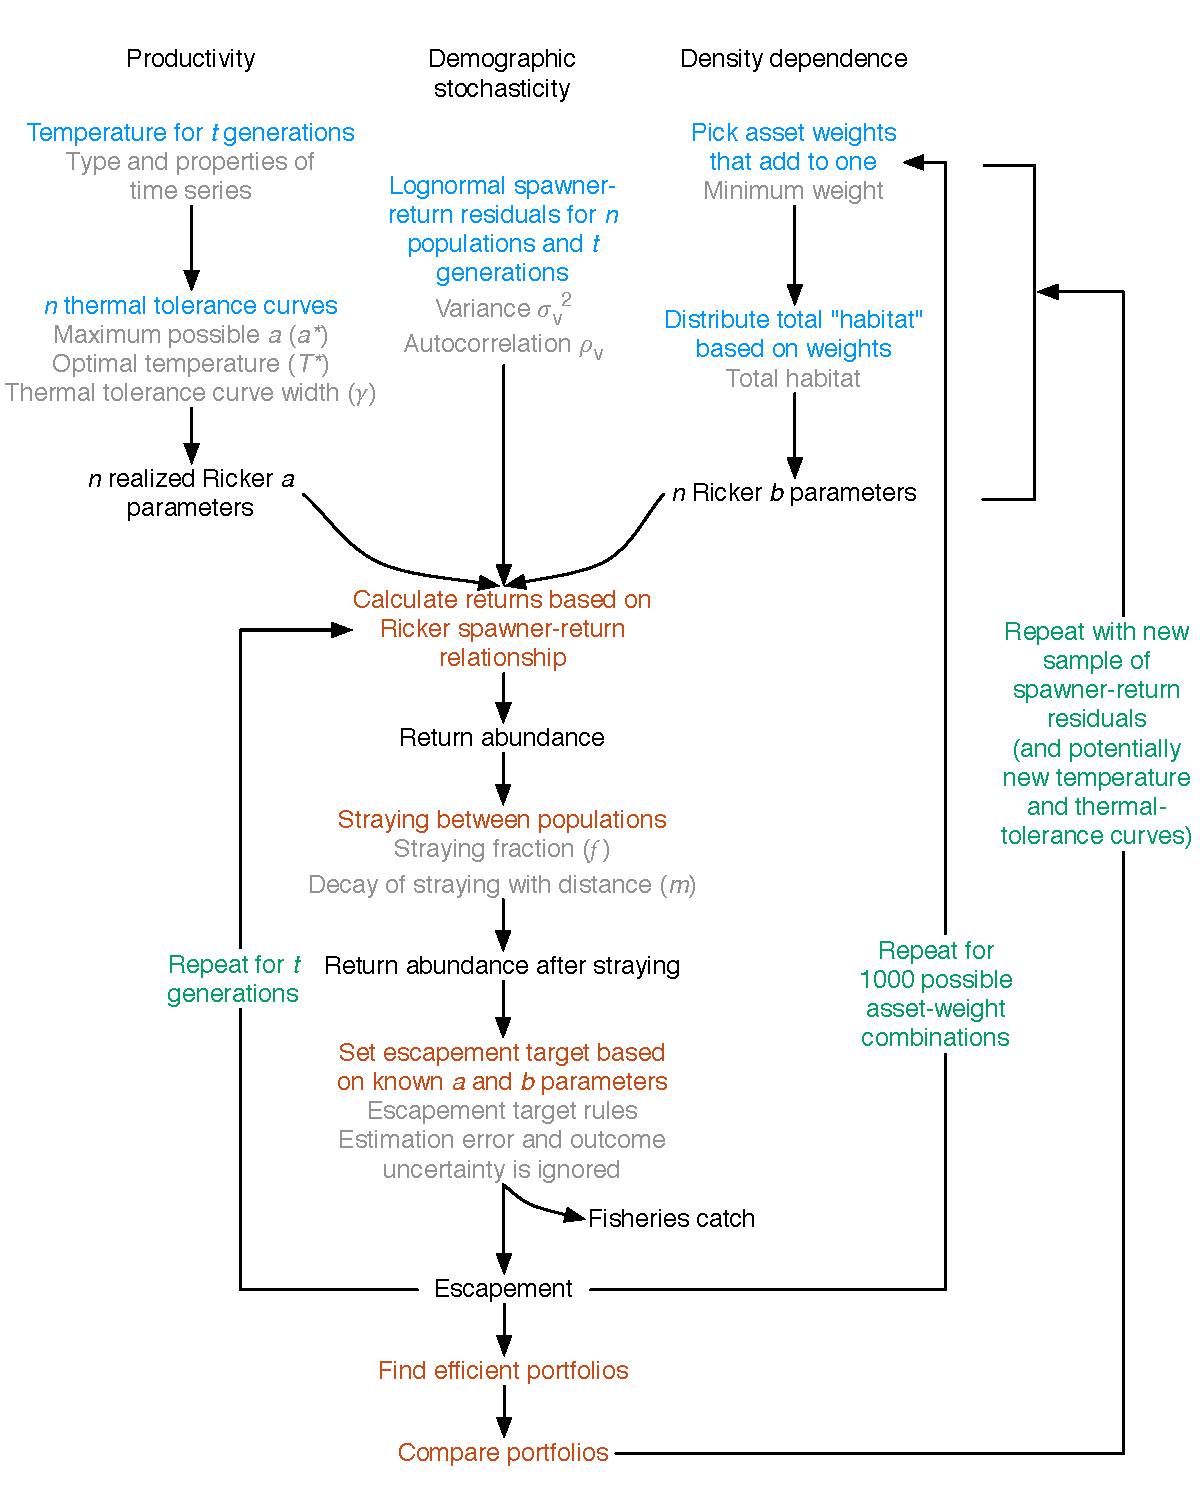
\includegraphics[height=6.5in]{simulation_diagram.pdf}
 \caption{Flow chart of the salmon-metapopulation simulation and portfolio optimization. There are $n$ salmon populations and $t$ generations. Blue text indicates values that are generated before the simulation progresses through time. Orange text indicates steps in which calculations are performed. Black text indicates values that are calculated. Grey text indicates parameters that can be set. Green text indicates the looping structure of the simulation.}
  \label{fig:sim-diagram}
\end{figure}

\subsection{Spawner-return relationship}

I am using a Ricker curve,

\begin{equation}
R_{ti} = S_{ti}e^{a_{ti}(1-S_{ti}/b_i) + w_{ti}},
\end{equation}

\noindent
where $t$ represents a generation time, $i$ represents a population, $R$
is the number of returns, $S$ is the number of spawners, $a$ is the
productivity parameter (which can vary with the environmental signal),
and $b$ is the density-dependent term (which is used as the asset
weights in the portfolios). The term $w_{ti}$ represents first-order
autocorrelated error (AR1). Formally,
$w_{ti} = w_{ti-1} \rho_w + v_{ti}$, where $v_{ti}$ represents
independent and normally distributed error with mean 0 and standard
deviation of $\sigma_v$. The parameter $\rho_w$ represents the
correlation between residuals from subsequent generations.

\subsection{Escapement targets}

I am calculating spawning abundance MSY $S_{MSY}$ each generation using
the equation $S_{MSY} = b(0.5-0.07a)$ from \citet{Hilborn1992} p272,
Table 7.2. I am using the precisely known $a$ and $b$ values each time
and assume perfect implementation of the escapement goal (no outcome
uncertainty) and no upper limit on how much the fishery can harvest. We
may want to add a bit of noise here, say by assuming a constant value
for $a$ or adding some implementation uncertainty. We need some level of
harvesting to keep the spawning population away from carrying capacity.
At carrying capacity, the productivity parameter $a$ has minimal effect
on population dynamics, making it a poor way to integrate response
diversity.

\subsection{Environmental signal}

I have programmed five different kinds of environmental signals. I think
it's easiest to think of these as temperature, but they could represent
more general environmental anomalies, such as the PDO. In Table
\ref{tab:env-types}, I describe the five kinds of environmental signals
I have included. Examples of these time series are illustrated in Figure
\ref{fig:env-ts}. Later, I may include black-swan-like events, although
the regime shifts could be seen this way if the changes are dramatic
enough. So far, all simulation results in the rest of this document use
a sine wave. The problem with using a randomly generated ARMA time
series is that you get much greater differences in the results from run
to run. This is fine in the long run, but hard to detect patterns
initially.

\begin{table}[h!]
\centering
\small
\caption{Environmental signals, parameters, and descriptions.}
\begin{tabular}{p{3.2cm}p{3.25cm}p{6.8cm}}
\toprule
Signal type & Parameters & Description \\
\midrule
Sine wave & $\overline{T} + A \cdot \sin(\omega t + \phi)$& $\overline{T}$ is 
the mean environmental value, $A$ is the amplitude, $\omega$ is the frequency in 
radians, and $\phi$ is the phase\\
ARMA & AR1, MA1, $\sigma_T$ & First-order autoregressive (AR1) and moving 
average (MA1) parameters and standard deviation; mean is assumed to be 0\\
Regime shifts & $T_{b0},T_{b1}, \ldots, T_{br-1}$; $T_{v0},T_{v1}, \ldots, T_{vr}$ 
& Breakpoints ($T_{b}$) and values ($T_v$) for regimes $1$ through $r$\\
Linear change & $T_{\mathrm{min}}$, $T_{\mathrm{max}}$ & Minimum and maximum 
values\\
Constant & $T_{\mathrm{constant}}$& Constant value\\
\bottomrule
\end{tabular}
\label{tab:env-types}
\end{table}

\begin{figure}[htbp]
\centering
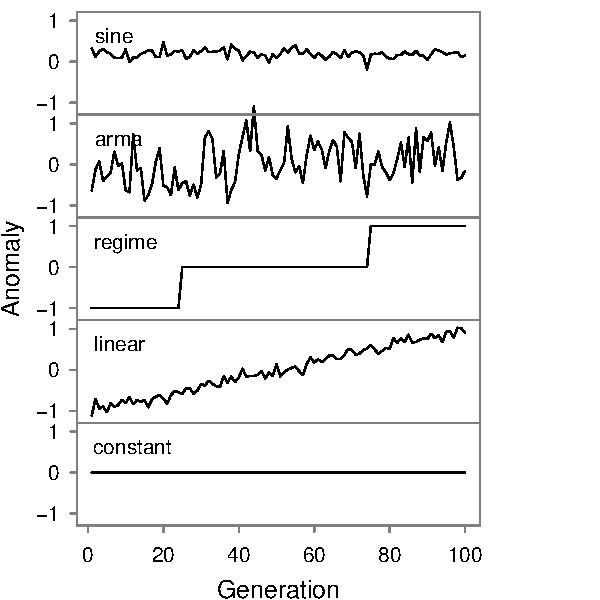
\includegraphics{figure/env-ts.pdf}
\caption{Example temperature time series\label{fig:env-ts}}
\end{figure}

\subsection{Straying}

{[}Insert a bit here about my research on straying and it's influence on
metapopulation dynamics for salmon{]}. Essentially, straying should be
enough to prevent local extinctions and ensure all possible habitat is
occupied, but probably not strong enough to noticeably affect population
dynamics or synchrony \citep{Schtickzelle2007}.

I've implemented straying as in \citet{Cooper1999}. I generate a matrix
that represents the fraction of straying between any two populations. I
have set up the metapopulation (thus far) in a very simple scenario: the
populations are arranged in a line and those that are nearer to each
other are more likely to stray between each other {[}insert caveats{]}.
Two parameters control the straying: the fraction of fish $f_{stray}$
that stray from their natal stream in any given generation and the rate
at which this straying between streams decays with distance $m$. I
calculated the number of salmon straying from stream $j$ to stream $i$
as,

\begin{equation}
  \mathrm{strays}_{tij} = f_{stray} R_{tj} \frac{e^{-m \lvert i-j \rvert }}{\displaystyle\sum\limits_{\substack{k = 1 \\
  k \neq j}}^{n} e^{-m \lvert k-j \rvert }},
\end{equation}

\noindent
where $R_{tj}$ is the number of returning salmon at generation $t$ whose
natal stream was stream $j$. The subscript $k$ represents a stream ID
and $n$ the number of populations. The denominator is a normalizing
constant to ensure the desired fraction of fish stray. See Figure
\ref{fig:stray-matrix} for an example straying matrix.

\begin{figure}[htbp]
\centering
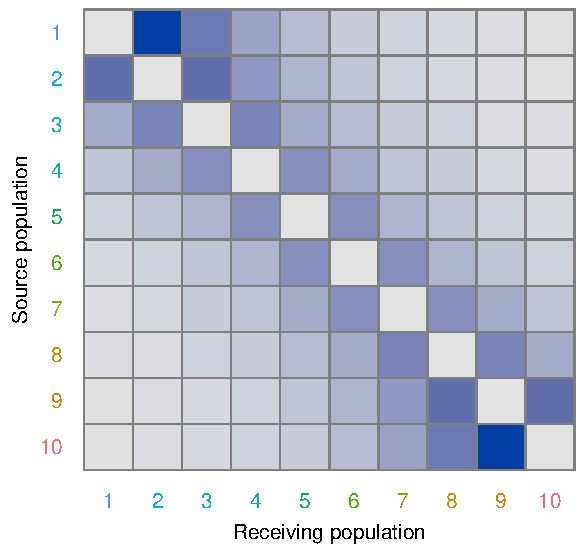
\includegraphics{figure/stray-matrix.pdf}
\caption{Example straying matrix. Darker blue colours indicate a greater
rate of straying.\label{fig:stray-matrix}}
\end{figure}

\subsection{Diversity of response to the environmental conditions}

{[}insert research I've done here on what can generate diversity of
response to the environment across populations and how it is typically
incorporated{]} This is a critical part to the paper.

I am incorporating diversity of response to environmental conditions,
say temperature, via changes in the Ricker $a$ parameter. I am using
thermal tolerance curves, based loosely on \citet{Eliason2011}. They
identify unique thermal tolerance curves in terms of cardiorespiratory
performance. I am using approximately the same temperature ranges and
variability of those curves, but applying them to productivity. I show
the curves I'm currently using in Figure \ref{fig:thermal-curves}. We
could vary the distribution of the optimum temperatures, the maximum $a$
values, and the width of the curves if we wanted, although I think the
current curves are a simple and straightforward base scenario and we may
not need to do anything more complicated.

I calculate $a_{ti}$, the realized Ricker productivity parameters after
accounting for thermal tolerance, as

\begin{equation}
  a_{ti} = a_i^* + \gamma_i (T_t - T_i^*)^2,
\end{equation}

\noindent
where $a_i^*$ is the maximum possible productivity parameter for
population $i$, $T_t$ is the temperature at time step $t$, $T_i^*$ is
the optimal temperature for population $i$, and $\gamma_i$ controls the
width of the thermal tolerance curve for each population. See Figure
\ref{fig:thermal-curves} for the default thermal tolerance curves for
ten populations.

Another possibility would be to draw the $a^*$, $\gamma$, and $T^*$
randomly. The advantage to setting it up as I have (with pre-specified
thermal tolerance curves) is that it will hopefully make the post-hoc
analysis of what affects the efficient frontier weights more
straightforward.

\begin{figure}[htbp]
\centering
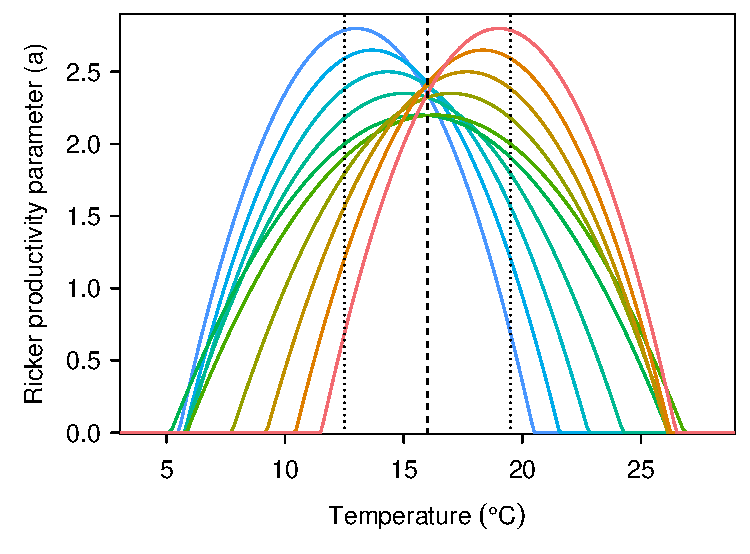
\includegraphics{figure/thermal-curves.pdf}
\caption{Thermal tolerance curves for ten populations. Here, and
throughout this document, I have used the same rainbow of colours to
identify the salmon populations. The populations are arranged from blue
(more productive with cooler temperatures) to red (more productive with
warmer temperatures). The vertical lines indicate mean, minimum, and
maximum values for one scenario --- you can ignore them for
now.\label{fig:thermal-curves}}
\end{figure}

\section{Summary of simulation parameters}

\begin{table}[h!]
\centering
\small
\caption{Salmon metapopulation parameters with base case and alternate values.}
\begin{tabular}{p{7.0cm}p{1.6cm}p{3.2cm}}
\toprule
Description & Parameter & Base [lower, upper] \\
\midrule
Stock-recruit residual standard deviation (on log scale) & $\sigma_v$ & 0.30 [0.05, 0.50] \\
First order (AR1) serial correlation of stock-recruit residuals & $\rho_w$ & 0.40 [0, 0.80] \\
Fraction of fish that stray from natal streams & $f_{stray}$ & 0.02 [0, 0.10] \\
Exponential rate of decay of straying with distance & $m$ & 0.30 [0.05, 0.50] \\
Standard deviation of beta distribution for implementation error & $\sigma_{impl}$ & 0.05 [0, 0.20] \\
Frequency of assessment (years) & $f_{assess}$ & 20 [5, 50] \\
\bottomrule
\end{tabular}
\label{tab:salm-pars}
\end{table}

\clearpage

\section{Portfolio optimization}

Details to follow. Quick version: I Monte Carlo the $b$ parameters (with
a specified minimum value) and measure the resulting mean and variance
of the rate of growth of the metapopulation salmon returns. I then
identify the set of $b$ parameters (i.e.~the set of weights) that
results in the efficient frontier. We could later choose to work with
risk metrics like conditional value at risk (CVaR), which measure the
probability of a ``bad'' event specifically, not the symmetrical
variance.

To find the efficient portfolios I divide all portfolios into bins by
mean rate of change and find the portfolios with the minimum variance
within each bin. I discard all portfolios with a mean rate of change
below the minimum variance portfolio. These are ``undesirable''
portfolios.

\section{Comparing portfolios}

This is a big area to think about. How do portfolios differ along the
frontier? How do the frontier portfolios differ from non-frontier
portfolios? What is the best way to visually compare them? What aspects
to compare? Are there summary statistics we could use to compare them?

\section{Some sample simulations}

\begin{figure}[htbp]
\centering
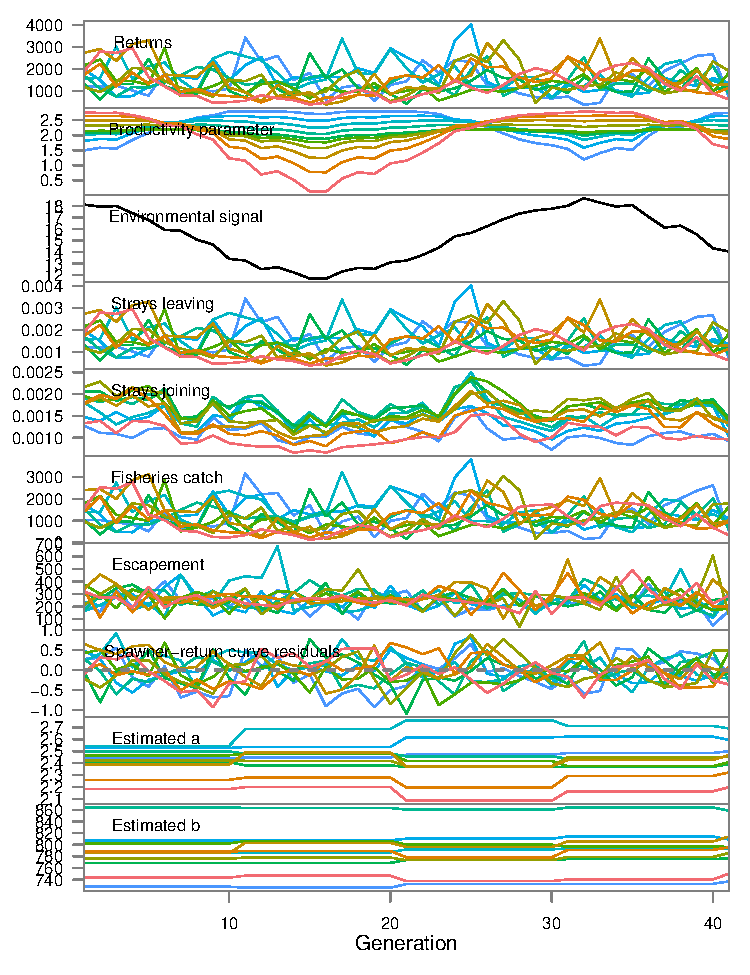
\includegraphics{figure/run-base-example1.pdf}
\caption{Example simulation with all parameters at default values. I'm
only showing a sample of 40 generations (after the burn-in period). From
top to bottom: salmon returns each generation (catch plus escapement);
Ricker $a$ parameter; the environmental signal (could think of it as
temperature or a composite environmental signal like the PDO); number of
salmon straying by population; number of straying salmon being received
by population; fisheries catch based on escapement MSY calculation;
salmon escapement; residuals from the spawner-return curve; estimated
Ricker $a$ parameter; estimated Ricker $b$ parameter.}
\end{figure}

\begin{figure}[htbp]
\centering
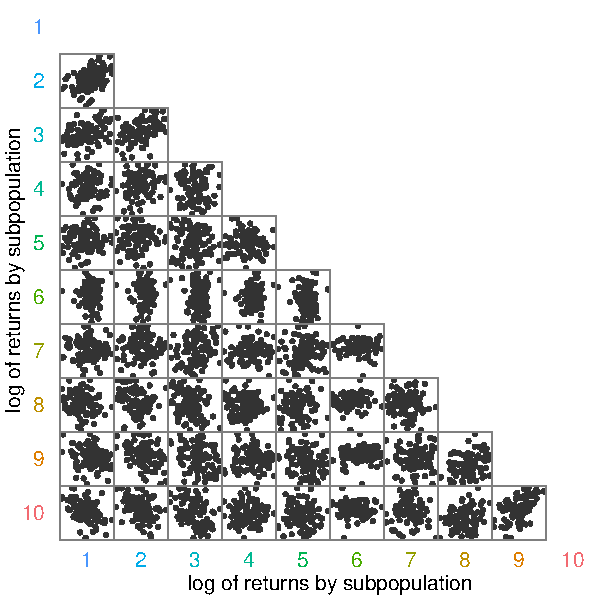
\includegraphics{figure/plot-base-corrs.pdf}
\caption{A plot comparing the log(returns) between each population. The
population colours and numbers match in all figures. Note how
populations 1 and 10 have asynchronous returns whereas populations with
more similar thermal-tolerance curves (say populations 9 and 10) have
more synchronous dynamics. Populations with thermal tolerance curves in
the middle (e.g.~population 6) are less correlated with other
populations. Their population dynamics end up primarily driven by
demographic stochasticity and less so by temperature-induced systematic
changes in productivity.}
\end{figure}

\begin{figure}[htbp]
\centering
\includegraphics{figure/plot-base-rickers.pdf}
\caption{We can also look at samples of the Ricker curves by population
(population numbers are in the upper left corners). Here, I've sampled
40 of the $a$ parameters through time for each population. The shaded
rectangles to indicate the range of spawners observed in the simulation.
The colour of the line indicates the temperature anomaly in that year
with blue indicating cooler years and red indicating warmer years. In
this example all the populations have the same $b$ parameters. Notice
how the productivity is more variable for populations nearer the limits
of their thermal tolerance (e.g.~population 1 vs.~population 5). Also
notice how population 1 is more productive in cool years whereas
population 10 is more productive in warm years.}
\end{figure}

\begin{figure}[htbp]
\centering
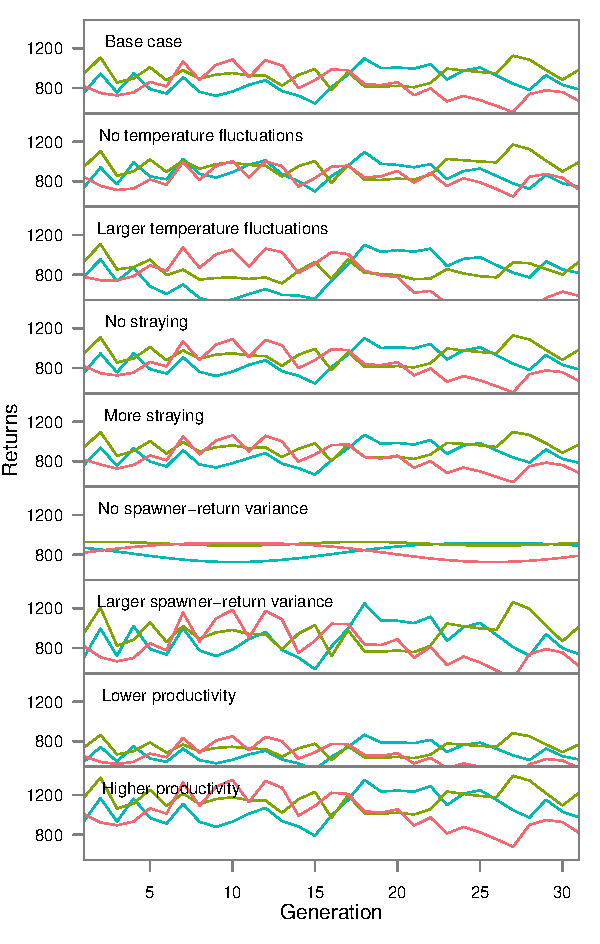
\includegraphics{figure/plot-various-options-ts-3pops.pdf}
\caption{Example simulations with different parameter values. I am
showing three populations here to make the plots easier to
interpret.\label{fig:sim-param-ts-3}}
\end{figure}

\clearpage

\section{An example of portfolio optimization}

Now, let's run an example where we find the $b$ values that form the
efficient frontier of metapopulation portfolios.

\begin{verbatim}
Error: ignoring SIGPIPE signal
\end{verbatim}

\begin{figure}[htbp]
\centering
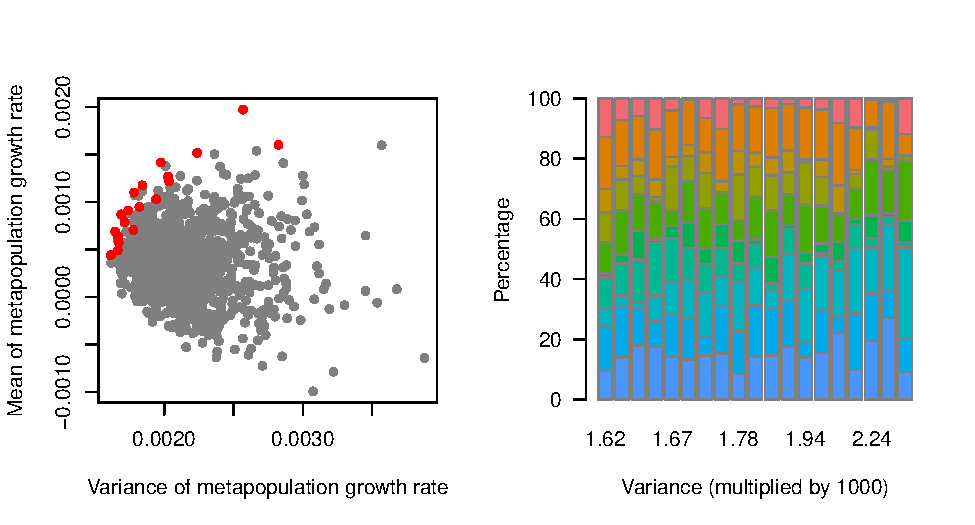
\includegraphics{figure/eff-frontier-eg.pdf}
\caption{Efficient frontier of metapopulation portfolios (red dots).
Each dot represents a different set of weights of the Ricker $b$
parameters. Metapopulation growth rate is the first difference of the
log of total metapopulation abundance. The colours in the right panel
correspond to the other figures.}
\end{figure}

\begin{figure}[htbp]
\centering
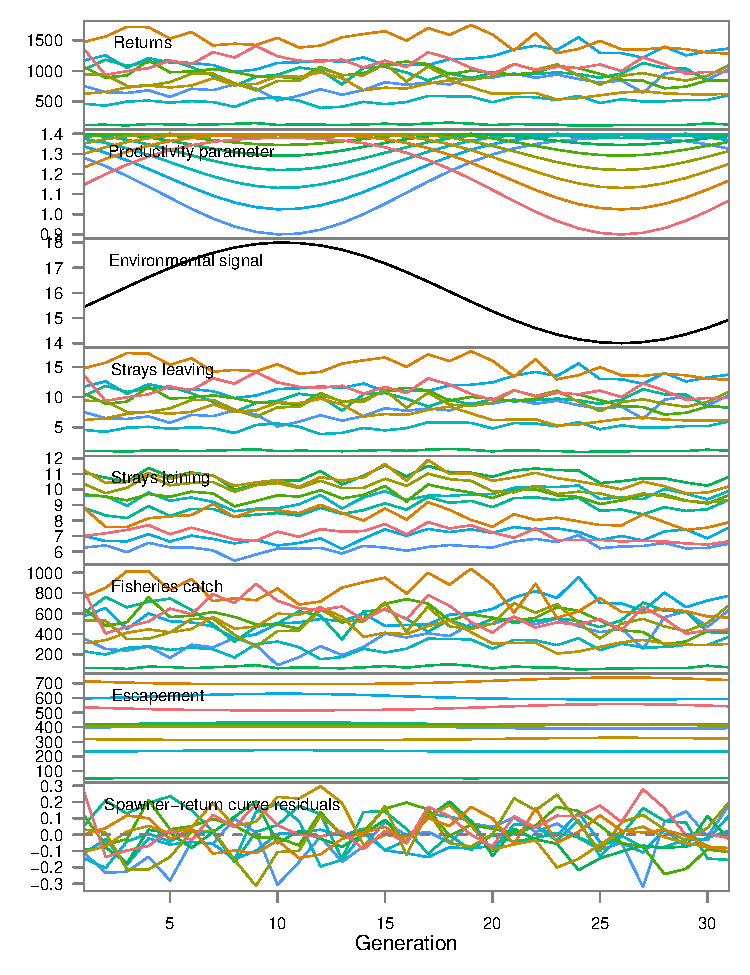
\includegraphics{figure/plot-eff-ports.pdf}
\caption{Simulation output from the minimum-variance metapopulation.}
\end{figure}

\begin{figure}[htbp]
\centering
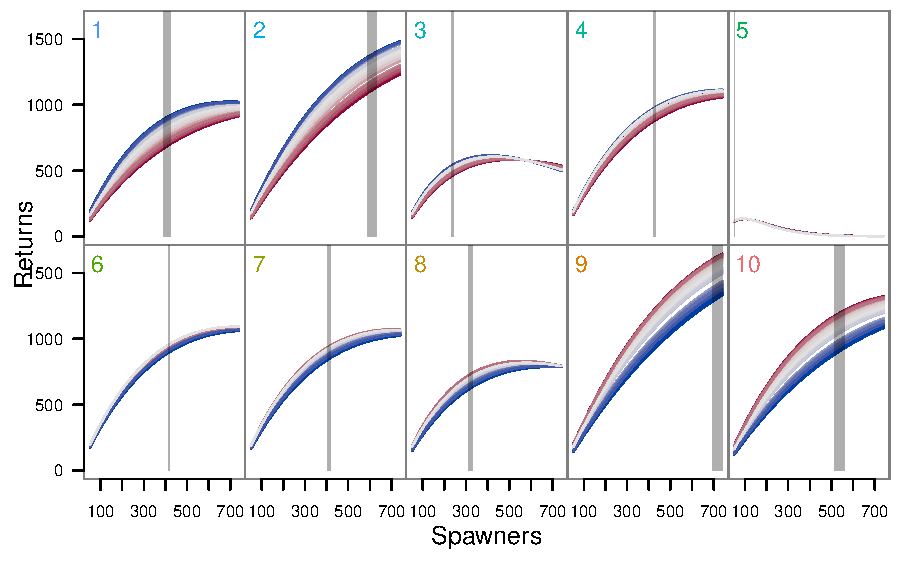
\includegraphics{figure/unnamed-chunk-1.pdf}
\caption{Example Ricker curves for the minimum-variance metapopulation.}
\end{figure}

\begin{figure}[htbp]
\centering
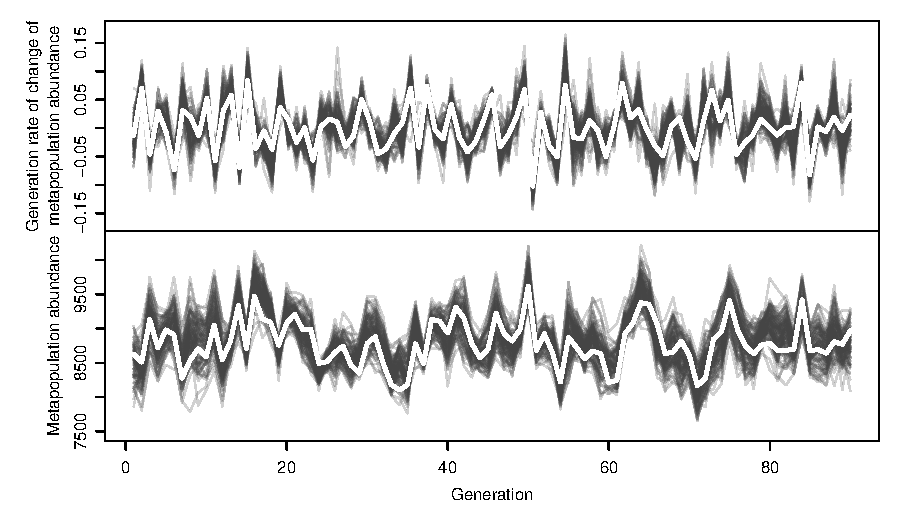
\includegraphics{figure/plot-portfolio-timeseries.pdf}
\caption{Time series for a random sample of portfolios (grey lines) and
the minimum-variance portfolio (white lines). The top panel shows rate
of change or metapopulation abundance at each time step and the bottom
panel shows the metapopulation abundance.}
\end{figure}

\begin{figure}[htbp]
\centering
\includegraphics{figure/plot-weights-samples.pdf}
\caption{A sample of 30 minimum-variance portfolios given the same set
of starting parameters as for the example illustrated above. The dashed
grey line indicates the weights if all populations had an equal carrying
capacity. As it stands, the weights look fairly random to me.}
\end{figure}

\begin{figure}[htbp]
\centering
\includegraphics{figure/plot-weights-median.pdf}
\caption{Median (solid line) and 25th and 75th quantiles of the weights
across 40 minimum-variance portfolios. Just another way of looking at
it.}
\end{figure}

\begin{figure}[htbp]
\centering
\includegraphics{figure/plot-cons-plans-curves.pdf}
\caption{Different ways of prioritizing conservation. The curves show
the environmental-tolerance curves for the populations that are
conserved. The colours are the same as earlier and identify the
different populations. These are in the same order as they are referred
to in the next two plots: full range of environmental response
diversity, most stable only, one half, other half, most asynchronous.}
\end{figure}

\begin{figure}[htbp]
\centering
\includegraphics{figure/plot-cons-plans-mv.pdf}
\caption{Conservation plans in mean-variance space. The dots show
portfolios from individual simulation runs. The dark and light shaded
areas show 25\% and 75\% quartiles. The left panel shows a scenario with
a stationary environmental signal and strong short-term environmental
noise. The right panel shows a scenario with a linearly-increasing
environmental signal and minimal short-term environmental noise. These
two scenarios bound the two environmental extremes: strong short-term
noise with minimal long-term signal vs.~a strong long-term signal with
minimal short-term signal. Notice what happens to the two \emph{half}
conservation strategies. A more realistic scenario combines the two. The
efficient frontier is shown for the displayed portfolios. This isn't
necessarily the overall efficient frontier.}
\end{figure}

\begin{figure}[htbp]
\centering
\includegraphics{figure/plot-cons-plans-ts.pdf}
\caption{Conservation plans in terms of metapopulation abundance. One
realization with a periodic (sine wave) environmental signal is shown as
an example. The light-grey lines in the background show 100
randomly-sampled portfolios with the same stock-recruit residuals and
the same environmental signal. Notice how much less variable the
scenarios with balanced response diversity are. The two scenarios with
unbalanced response diversity tend to seesaw with the environment.}
\end{figure}

\clearpage

\section{Take home messages}

\begin{enumerate}
\def\labelenumi{\arabic{enumi}.}
\itemsep1pt\parskip0pt\parsep0pt
\item
  If the dominant environmental signal is a long-term shift, and you
  keep around one half of the response diversity, then you get different
  portfolio means but the same variances.
\item
  If the dominant environmental signal is short-term, and you keep
  around one half of the response diversity, then you get different
  portfolio variances but the same means.
\item
  Combine those two (which best reflects reality) and you get both
  different means and variances.
\item
  Whether you invest in just stable, just asynchronous, or a mix of
  both, all that really matters is that you have as many populations as
  possible and as balanced as possible response diversity.
\item
  An even weighting across as many possible streams (assuming balanced
  response diversity) gets you pretty close to the minimum-variance
  portfolio. {[}not shown currently{]}
\item
  With systematic long-term environmental change that dominates: if you
  can forecast the environment and know the responses of salmon
  populations from individual streams then you can increase your
  expected rate of metapopulation growth with minimal effect on variance
  by prioritizing the populations that will do well. Although if you get
  it wrong you will do worse than if you had hedged your bets and
  conserved response diversity.
\item
  But, if there are also strong short-term environmental fluctuations
  (and there probably are), then there's always a benefit to portfolio
  variance by having some response diversity.
\item
  Variable stocks aren't inherently undesirable to conserve, as long as
  they are balanced or averaged out.
\item
  Take home message: ``To keep every cog and wheel is the first
  precaution of intelligent tinkering.'' But, if you must prioritize,
  keep a selection of different cogs and wheels --- especially a
  spatially diverse set of cogs and wheels. That gives you the best
  chance of an efficient ecological portfolio.
\end{enumerate}

\section{Open questions and next steps}

\begin{enumerate}
\def\labelenumi{\arabic{enumi}.}
\itemsep1pt\parskip0pt\parsep0pt
\item
  How do smaller or larger values of the various parameters affect the
  results?
\item
  Are the results sensitive to the height and width of the thermal
  tolerance curves? (I think within reason, no.)
\item
  Are these results robust to, say, cyclical or regime shift style
  environmental noise?
\item
  Should this be a generic ``environmental signal'' or temperature?
\item
  Show what happens for a given scenario as you conserve more streams
  (it gets closer to the minimum-variance portfolio).
\item
  Show an example of where these conservation plans place you in
  mean-variance space across all possible weights. (Done but not shown.)
\item
  Bring these conservation plans back to established suggestions
  (e.g.~VSP).
\item
  How can we simplify the main figures?
\item
  Is there a way to combine the main figures to make the result more
  understandable (e.g.~little response-diversity curves as a legend)?
\item
  Redo the Monte Carlo portfolios to show an extreme example where you
  can see the weights shifting. For example, a linearly increasing
  environmental signal with some generation-to-generation noise.
\item
  Generations or years? Years seem simpler to talk about. Generations
  seem more widely applicable and accurate.
\end{enumerate}

\clearpage

\renewcommand\refname{References}
\bibliography{jshort,salmonport}

\end{document}
